\section{Results}
\label{sec:results}
Our experiments did not yield as many viable chairs as we had hoped, nor did
they yield truly novel designs. They did however produce some interesting
individuals, and reveal entertaining problems in our simulations.
This section details our results, and our understanding and interpretation of
how and why they occurred. The next section, we go further in depth with
understanding and interpretation of our results, and discuss what might be
changed to produce better chairs.

Several experiments were performed using the evaluation
function mentioned in section \ref{sec:evaluation}. Most of the experiments 
where carried out with a population size of 50 and a species count of 10. 
However, in an attempt to reach later generations, some experiments were 
carried out using only a population size of 10 and a species count of 2.

Initially the experiments were carried out without the interactive term, $I$,
and without regard for the mass of the individuals produced by the EC. This
meant that the physical part of the evaluation, where Ethan was dropped on the
individuals, resulted in the terms, $E_\Delta$, $E_{rest}$, and $E_{posture}$
all being roughly equivalent between individuals. This happened because the
comparatively high mass of Ethan would always result in the individuals being
rotated and Ethan dropping on the floor. This left only the $|V|$ and $R_c$
terms, and the EC ultimately optimized towards a minimal voxel count which would
not rotate when Ethan was dropped, see figure~\ref{fig:flat_object}.

\begin{figure}[ht]
\centering
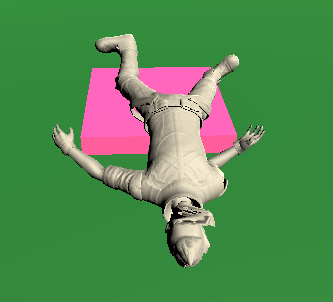
\includegraphics[scale=.5]{flat_chair}
\caption{The evolved individual, pink, is simply a flat structure, such that
it does not rotate when Ethan is dropped on it, and has minimal voxel
count.} \label{fig:flat_object} 
\end{figure}

Adding the interactive term, $I$, did not improve significantly on the above
results. While the selected individual would persist through several
generations, the other best performing individuals would still optimize towards
the aforementioned flat structure, see figure~\ref{fig:selection}.
\begin{figure}[ht]
	\centering
	\subfloat[]{
		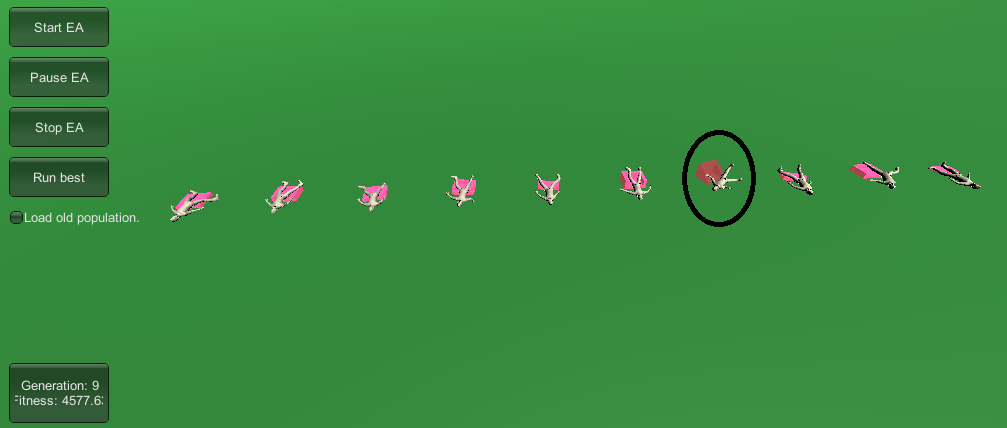
\includegraphics[width=.9\columnwidth, trim={110 0 0 0}, clip]{selection}
	} \hfil
	\subfloat[]{
		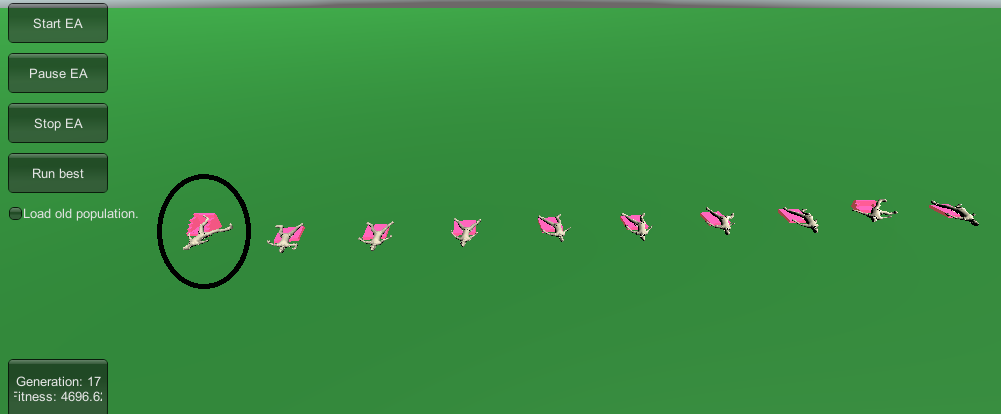
\includegraphics[width=.9\columnwidth, trim={110 0 0 0}, clip]{selection2}
	}
	\caption{Example showing how the selected individual, encircled in (a),
	persists 8 generations later, encircled in (b).} \label{fig:selection}
\end{figure}

Further experiments were conducted, where the mass of the individuals was
adjusted according to their voxel count. In these experiments the EC ended up
producing some individuals which were not just flat individuals. Rather it produced
individuals as boxes on which Ethan could rest in a height such that the terms
$E_{rest}$ and $E_\Delta$ were minimized, see figure~\ref{fig:boxchair}.

\begin{figure}[ht]
	\centering
	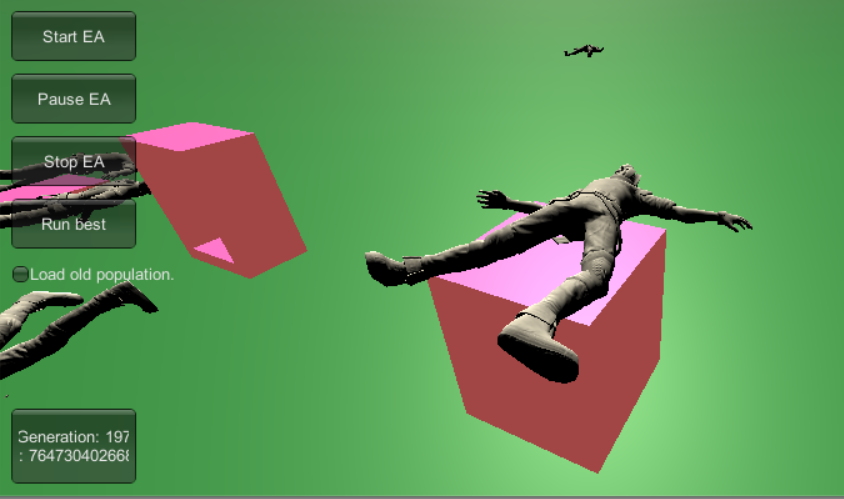
\includegraphics[width=.9\columnwidth, trim={110 0 0 65}, clip]{box_chair}
	\caption{When considering the mass of the individuals, such that more
	compact individuals are more sturdy, the EC evolved a box upon which
	Ethan could rest.}
	\label{fig:boxchair}
\end{figure}

\begin{figure}[ht]
	\centering
	\subfloat[]{
		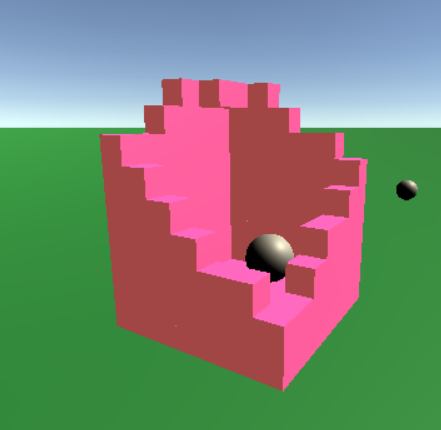
\includegraphics[height=130pt]{basket}
	} \hfil
	\subfloat[]{
		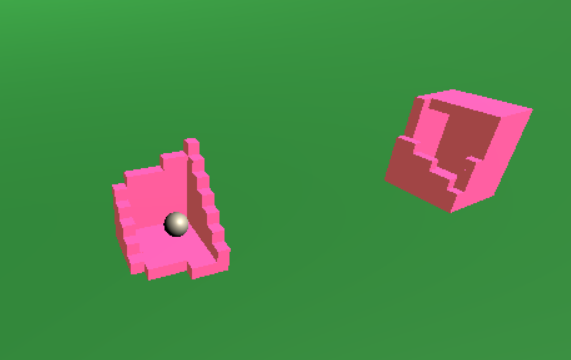
\includegraphics[width=.9\columnwidth]{basket2}
	}
	\caption{Basket like shapes that might have functioned as chairs, had
	they had legs.}
	\label{fig:baskets}
\end{figure}

Exchanging Ethan experiments with spheres, we saw some promising results. The
mat- and tray-like shapes we had been seeing took on more basket-like shapes,
reminiscent of bean bag chairs. We believe that with more generations, they
might have started to grow in height --- perhaps with legs. Figure
\ref{fig:baskets} depicts some basket-like shapes.

\begin{figure}[ht]
	\centering
	\subfloat[]{
		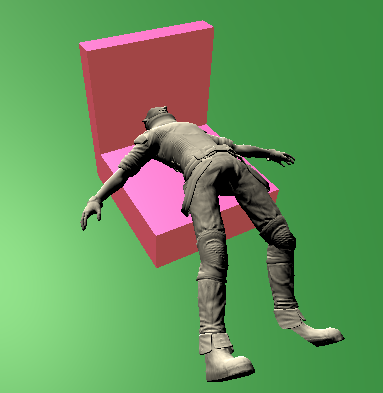
\includegraphics[height=130pt]{actual_chair}
		\label{fig:real_chair}
	} \hfil
	\subfloat[]{
		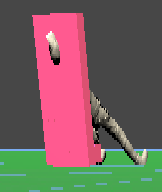
\includegraphics[height=110pt]{metro_stand}
		\label{fig:metro_stand}
	}
	\subfloat[]{
	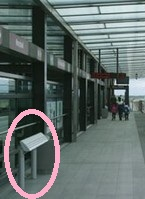
\includegraphics[height=110pt]{metro_stand_real}
		\label{fig:metro_stand_real}
	}
	\caption{Two viable chairs. While the topmost chair is nothing more than
	viable, the bottom-left chair is a little surprising. Bottom-right is a
	photograph of the rests found at metro platforms in Copenhagen}
	\label{fig:viable_chairs}
\end{figure}

We did see some viable chairs --- individuals that a person could use for seating.
Figure \ref{fig:real_chair} shows an example, not unlike a car seat. A more
surprising result can be seen in figure \ref{fig:metro_stand}. The chair bares
resemblance to the rests that can be found at metro platforms in Copenhagen, and
is an interesting diversion from common chair morphologies. An example of such 
a rest can be seen in figure \ref{fig:metro_stand_real}. It is debatable 
whether an individual one leans on can be considered a chair, but it suits the 
fitness function.

Some chair-like individuals were unfairly evaluated in simulation. Because the
simulation of "sitting" is simplified, some individuals were missed or even
toppled over in simulation. Figure \ref{fig:footstools} shows some chair-like
individuals that ended up as strange footstools. Even the seat-like individual
in figure \ref{fig:viable_chairs} is misjudged by Ethan not being able to sit up
straight (although as one author commented; \emph{"That's how I sit"}).

Another potential branch of candidates, as seen in the third physics video\cite{vid:video3}, is frame like structures.
These seem to develop by minimizing the voxel count and stability is maximized by actually not colliding with the drop object.
Later generations could potentially generate a flat surface which would increase the height of 
where the drop object comes to a rest and the rectangular frame could provide grounds for legs. 

\begin{figure}[ht]
	\centering
	\subfloat[]{
		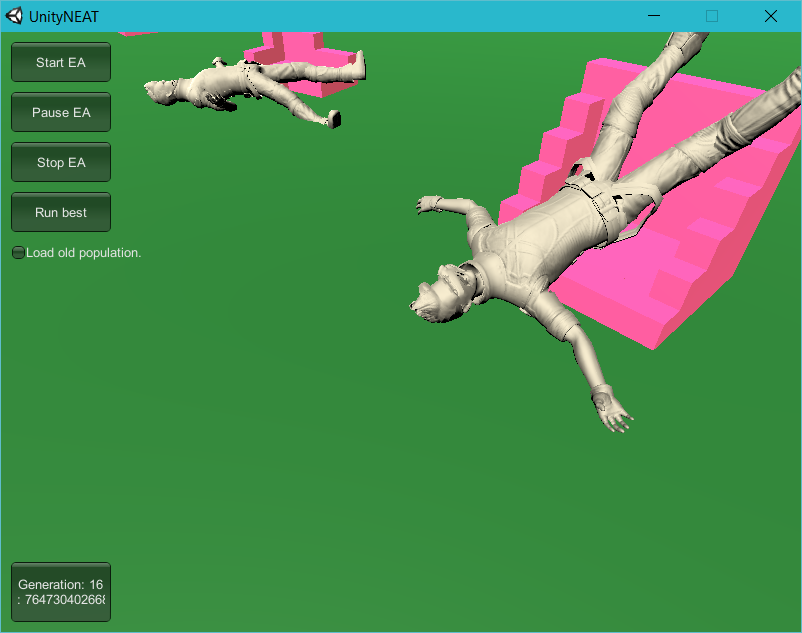
\includegraphics[width=0.4\columnwidth, trim={130 70 0 20}, clip]{chair_flipover} } \hfil
	\subfloat[]{
		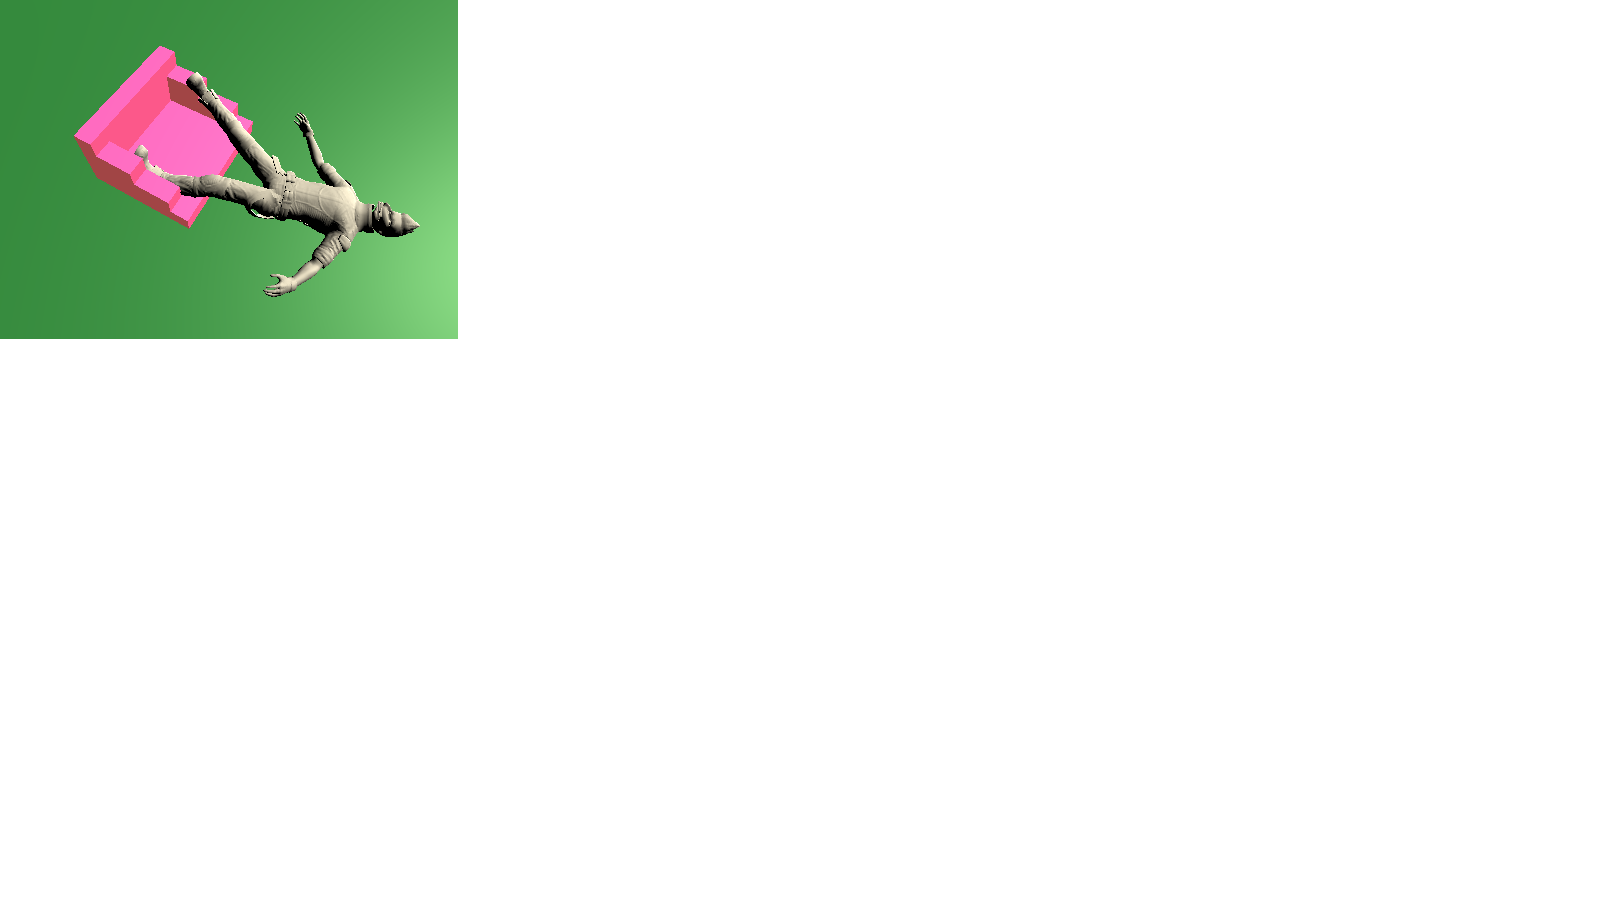
\includegraphics[width=0.4\columnwidth, trim={30 0 0 0}, clip]{footstool}
	}
	\caption{The simulation is not entirely loyal to reality. Viable chairs
	might be deemed unfit because "sitting" is imperfectly simulated.}
	\label{fig:footstools}
\end{figure}

\begin{figure}[h]
\centering
\subfloat[]{
	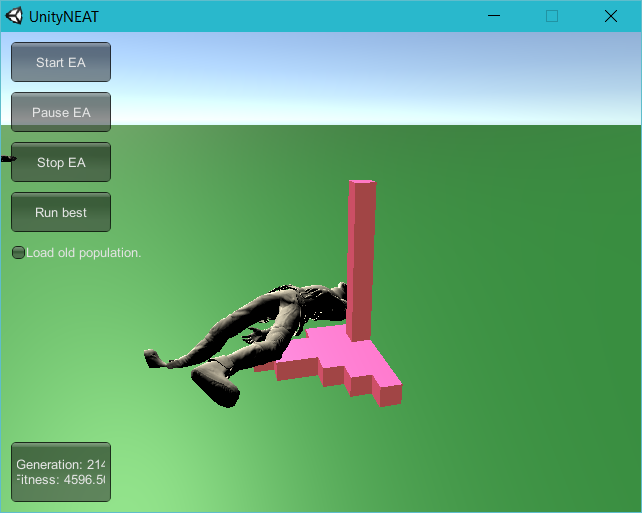
\includegraphics[width=.4\columnwidth, trim={80 0 80 60}, clip]{chair_leg}
}
\hfil
\subfloat[]{
	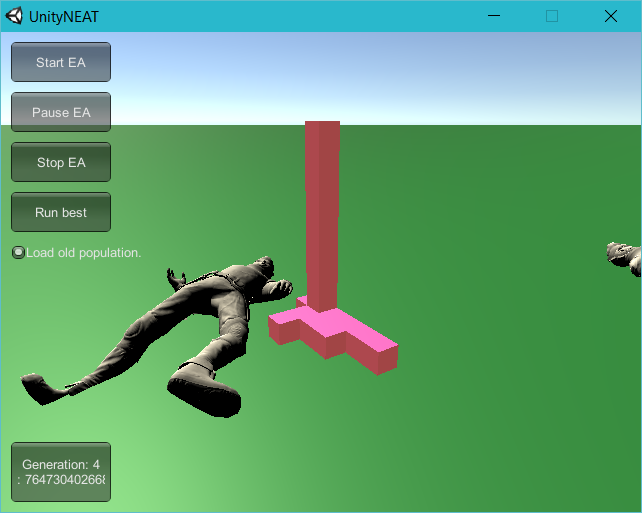
\includegraphics[width=.4\columnwidth, trim={80 20 80 40}, clip]{chair_leg2}
}
\caption{Asymmetric shapes, that may have evolved into chair legs}
\label{fig:chair_legs}
\end{figure}

While we never saw individuals with a sitting-surface lifted up on legs, the
experiments did evolve morphologies that might have become legs in later
generations. The morphologies in figure \ref{fig:chair_legs} are asymmetric
leg-like support structures. We believe they where selected for, because they
provide momentary support for Ethan as he falls on them, until he falls to the
side. As such, they may not have evolved as legs, but if arranged into a
symmetric grid, they could have carried some of the viable chair morphologies we
have seen, producing lower $E_{rest}$ terms in the evaluation of those
individuals, and hence a higher fitness.
